\lstset{ %
	language=python,                % Язык программирования                % где поставить нумерацию строк (слева\справа)
	numberstyle=\tiny,           % размер шрифта для номеров строк
	stepnumber=1,                   % размер шага между двумя номерами строк
	numbersep=5pt,                % как далеко отстоят номера строк от подсвечиваемого кода
	showspaces=false,            % показывать или нет пробелы специальными отступами
	showstringspaces=false,      % показывать или нет пробелы в строках
	showtabs=false,             % показывать или нет табуляцию в строках
	tabsize=2,                 % размер табуляции по умолчанию равен 2 пробелам
	captionpos=t,              % позиция заголовка вверху [t] или внизу [b] 
	breaklines=true,           % автоматически переносить строки (да\нет)
	breakatwhitespace=false,       
	frame=single,                    % Добавить рамку
	basicstyle=\small,
	escapebegin=\begin{russian}\commentfont,
		escapeend=\end{russian},
	literate={Ö}{{\"O}}1
	{Ä}{{\"A}}1
	{Ü}{{\"U}}1
	{ß}{{\ss}}1
	{ü}{{\"u}}1
	{ä}{{\"a}}1
	{ö}{{\"o}}1
	{~}{{\textasciitilde}}1
	{а}{{\selectfont\char224}}1
	{б}{{\selectfont\char225}}1
	{в}{{\selectfont\char226}}1
	{г}{{\selectfont\char227}}1
	{д}{{\selectfont\char228}}1
	{е}{{\selectfont\char229}}1
	{ё}{{\"e}}1
	{ж}{{\selectfont\char230}}1
	{з}{{\selectfont\char231}}1
	{и}{{\selectfont\char232}}1
	{й}{{\selectfont\char233}}1
	{к}{{\selectfont\char234}}1
	{л}{{\selectfont\char235}}1
	{м}{{\selectfont\char236}}1
	{н}{{\selectfont\char237}}1
	{о}{{\selectfont\char238}}1
	{п}{{\selectfont\char239}}1
	{р}{{\selectfont\char240}}1
	{с}{{\selectfont\char241}}1
	{т}{{\selectfont\char242}}1
	{у}{{\selectfont\char243}}1
	{ф}{{\selectfont\char244}}1
	{х}{{\selectfont\char245}}1
	{ц}{{\selectfont\char246}}1
	{ч}{{\selectfont\char247}}1
	{ш}{{\selectfont\char248}}1
	{щ}{{\selectfont\char249}}1
	{ъ}{{\selectfont\char250}}1
	{ы}{{\selectfont\char251}}1
	{ь}{{\selectfont\char252}}1
	{э}{{\selectfont\char253}}1
	{ю}{{\selectfont\char254}}1
	{я}{{\selectfont\char255}}1
	{А}{{\selectfont\char192}}1
	{Б}{{\selectfont\char193}}1
	{В}{{\selectfont\char194}}1
	{Г}{{\selectfont\char195}}1
	{Д}{{\selectfont\char196}}1
	{Е}{{\selectfont\char197}}1
	{Ё}{{\"E}}1
	{Ж}{{\selectfont\char198}}1
	{З}{{\selectfont\char199}}1
	{И}{{\selectfont\char200}}1
	{Й}{{\selectfont\char201}}1
	{К}{{\selectfont\char202}}1
	{Л}{{\selectfont\char203}}1
	{М}{{\selectfont\char204}}1
	{Н}{{\selectfont\char205}}1
	{О}{{\selectfont\char206}}1
	{П}{{\selectfont\char207}}1
	{Р}{{\selectfont\char208}}1
	{С}{{\selectfont\char209}}1
	{Т}{{\selectfont\char210}}1
	{У}{{\selectfont\char211}}1
	{Ф}{{\selectfont\char212}}1
	{Х}{{\selectfont\char213}}1
	{Ц}{{\selectfont\char214}}1
	{Ч}{{\selectfont\char215}}1
	{Ш}{{\selectfont\char216}}1
	{Щ}{{\selectfont\char217}}1
	{Ъ}{{\selectfont\char218}}1
	{Ы}{{\selectfont\char219}}1
	{Ь}{{\selectfont\char220}}1
	{Э}{{\selectfont\char221}}1
	{Ю}{{\selectfont\char222}}1
	{Я}{{\selectfont\char223}}1
	{і}{{\selectfont\char105}}1
	{ї}{{\selectfont\char168}}1
	{є}{{\selectfont\char185}}1
	{ґ}{{\selectfont\char160}}1
	{І}{{\selectfont\char73}}1
	{Ї}{{\selectfont\char136}}1
	{Є}{{\selectfont\char153}}1
	{Ґ}{{\selectfont\char128}}1
}
\newpage
\Large
\section*{Реферат}%
\addcontentsline{toc}{section}{\tocsecindent{Реферат}}

Расчетно-пояснительная записка содержит 30 стр., 5 рис., 4 листинга и 4 источника.

Ключевые слова: LaTeX, библиотека, проектирование, база данных, web, MS-SQL, веб-приложение, Web.

Курсовой проект представляет собой веб-приложение, в котором пользователь может создавать список литературы из книг, содержащихся в библиотеке.

В данной работе были рассмотрены различные подходы к хранению данных в БД.

Использовался язык программирования Python с библиотеками pyodbc и Dash.
\newpage
\section*{Введение}%
\addcontentsline{toc}{section}{\tocsecindent{Введение}}

При написании отчета в среде LaTeX, когда доходит дело до составления списка литературы, у многих возникают сложности связанные с тем, что в LaTeX не предусмотрен автоматический способ генерации элементов списка литературы, и все приходится писать вручную, что довольно муторно и высока вероятность допустить ошибку. Поэтому в этой работе были поставлены задачи:
\begin{enumerate}
	\item проанализировать существующие на рынке СУБД и выбрать наиболее подходящую для реализации библиотеки;
	\item спроектировать базу данных для хранения информации об источниках информации;
	\item реализовать web-приложение, позволяющее автоматически генерировать список литературы;
	\item и наконец, провести тестирование и проверить работоспособность разработанного приложения.

\end{enumerate}\newpage
\section*{Аналитическая часть}%
\addcontentsline{toc}{section}{\tocsecindent{Аналитическая часть}}

В данном разделе будут рассмотрены общие сведения о БД и СУБД, типы БД и используемые framework. 

\subsection*{Формализация задачи}%
\addcontentsline{toc}{subsection}{\tocsecindent{Постановка задачи}}

В соответствии с техническим заданием на курсовой проект, требуется создать базу данных для хранения книг в библиотеке, при этом должна быть предусмотрена возможность просмотра содержимого этой библиотеки.

Также требуется реализовать web-приложение, позволяющее создавать файл списка литературы и осуществлять просмотр содержимого библиотеки.

\subsection*{Общие сведения о БД  СУБД}%
\addcontentsline{toc}{subsection}{\tocsecindent{Общие сведения о БД  СУБД}}
База данных представляет собой совокупность определенным образом организованных данных, которые хранятся в памяти вычислительной системы и отображают состояние объектов и их взаимосвязи в рассматриваемой предметной области.\\
Под системой управления базами данных \(СУБД\) понимается совокупность программных и языковых средств, предназначенных для создания и обработки БД. 

\subsection*{Типы БД}
\addcontentsline{toc}{subsection}{\tocsecindent{Типы БД}}

Модель данных определяет логическую структуру БД и то, каким образом данные будут храниться, организовываться и обрабатываться. 

Существует 3 типа моделей организации данных:
\begin{itemize}
	\item иерархическая модель БД;
	\item сетевая модель БД;
	\item реляционная модель.
\end{itemize}

\subsubsection*{Иерархическая модель БД}
\addcontentsline{toc}{subsection}{\tocsecindent{Иерархическая модель БД}}

Иерархическая модель БД представляет собой древовидную (иерархическую) структуру, состоящую из объектов (данных) различных уровней. Каждый объект может включать в себя несколько объектов более низкого уровня. Такие объекты находятся в отношении предка (объект более близкий к корню) к потомку (объект более низкого уровня), при этом возможна ситуация, когда объект-предок имеет несколько потомков, тогда как у объекта-потомка обязателен только один предок.

Иерархической базой данных является файловая система, состоящая из корневого каталога, в котором имеется иерархия подкаталогов и файлов.

Связи записей реализуются в виде физических указателей с одной записи на другую. Основной недостаток иерархической структуры – невозможность реализовать отношения "многие-ко-многим", а также ситуации, в которых запись имеет несколько предков. \cite{litlink1}

\subsubsection*{Сетевая модель}
\addcontentsline{toc}{subsection}{\tocsecindent{Сетевая модель}}
Сетевая модель данных является расширением иерархического подхода. 
Разница между иерархической моделью данных и сетевой заключается в том, что в иерархических структурах запись-потомок должна иметь в точности одного предка, а в сетевой структуре у потомка может быть любое число предков. 
Записи в такой модели связаны списками с указателями.

Примером сетевой СУБД является IDMS (интегрированная система управления данными) от компании Computer Associates international Inc.

Популярность сетевой модели совпала с популярностью иерархической модели. 
Некоторые данные намного естественнее моделировать с несколькими предками для одного дочернего элемента. 
Сетевая модель позволяла моделировать отношения «многие-ко-многим».

И хотя эта модель широко применялась на практике, она так и не стала доминантной по двум основным причинам. 
Во-первых, компания IBM решила не отказываться от иерархической модели в расширениях для своих продуктов, таких как IMS и DL/I. 
Во-вторых, через некоторое время ее сменила реляционная модель, предлагавшая более высокоуровневый, декларативный интерфейс. \cite{litlink1}

\subsubsection*{Реляционная модель}
\addcontentsline{toc}{subsection}{\tocsecindent{Реляционная модель}}

В реляционной модели, в отличие от иерархической или сетевой, не существует физических отношений. Вся информация хранится в виде таблиц (отношений), состоящих из рядов и столбцов. А данные двух таблиц связаны общими столбцами, а не физическими ссылками или указателями. Объекты и их отношения представлены таблицами.

В реляционных моделях нет необходимости просматривать все указатели, что облегчает выполнение запросов на выборку информации по сравнению с сетевыми и иерархическими БД. Это одна из основных причин, почему реляционная модель оказалась более удобна.

Самые распространенные реляционные СУБД: MySql, PostgreSql, Access, Oracle, DB2, MS-SQL Server, SQLite.
Каждая реляционная таблица представляет собой двумерный массив и обладает следующими свойствами:

\begin{enumerate}
	\item каждый элемент таблицы — один элемент данных;
	\item все элементы в одном столбце имеют одинаковый тип;
	\item каждый столбец имеет уникальное имя;
	\item одинаковые строки (записи, кортежи) в таблице отсутствуют;
	\item порядок следования строк и столбцов может быть произвольным.
\end{enumerate}


Каждое поле содержит одну характеристику объекта предметной области. В записи собраны сведения об одном экземпляре этого объекта.

Некоторые поля могут быть определены как ключевые. Это значит, что для ускорения поиска конкретных значений будет использоваться индексация. Когда поля двух различных таблиц получают данные из одного набора, можно использовать оператор JOIN для выбора связанных записей двух таблиц, сопоставив значения полей. Такие действия можно расширить до объединения нескольких полей в нескольких таблицах. Поскольку отношения здесь определяются только временем поиска, реляционные базы данных классифицируются как динамические системы. 

\subsubsection*{Сравнение моделей}
\addcontentsline{toc}{subsection}{\tocsecindent{Сравнение моделей}}

Иерархическая модель данных поддерживает отношения типа «один-к-одному» или «один-ко-многим». Она позволяет быстро получать данные, но не отличается гибкостью. Иногда роль элемента (родителя или потомка) неясна и не подходит для иерархической модели.

Вторая, сетевая модель данных, имеет более гибкую структуру, чем иерархическая, и поддерживает отношение «многие ко многим». Но быстро становится слишком сложной и неудобной для управления.

Третья модель – реляционная – более гибкая, чем иерархическая и проще для управления, чем сетевая. Реляционная модель сегодня используется чаще всего, так как имеет множество преимуществ, таких как:

\begin{enumerate}
	\item простота использования;
	\item гибкость;
	\item независимость данных;
	\item безопасность;
	\item простота практического применения;
	\item слияние данных;
	\item целостность данных.
\end{enumerate}

В связи с этим, далее будет рассматриваться реляционная модель. Осталось только рассмотреть систему управления такой моделью.

\subsection*{СУБД}%
\addcontentsline{toc}{subsection}{\tocsecindent{СУБД}}

Среди самых популярных систем управления реляционными базами данных:
\begin{enumerate}
	\item MS-SQL Server;
	\item MySQL;
	\item PostgreSQL; 
	\item SQLite.
\end{enumerate}

В данном проекте будет рассмотрела СУБД MS-SQL Server.

SQL Server является одной из наиболее популярных систем управления базами данных (СУБД) в мире. Данная СУБД подходит для самых различных проектов: от небольших приложений до больших высоконагруженных проектов.

SQL Server был создан компанией Microsoft. Первая версия вышла в 1987 году. А текущей версией является версия 16, которая вышла в 2016 году и которая будет использоваться в текущем руководстве.

SQL Server долгое время был исключительно системой управления базами данных для Windows, однако начиная с версии 16 эта система доступна и на Linux \cite{litlink2}. 

Преимущества:

\begin{enumerate}
	\item \textbf{Производительность.} SQL Server работает очень быстро.
	\item \textbf{Надежность и безопасность.} SQL Server предоставляет шифрование данных.
	\item \textbf{Простота.}  С данной СУБД относительно легко работать и вести администрирование.
\end{enumerate}

\subsection*{Framework}%
\addcontentsline{toc}{subsection}{\tocsecindent{Framework}}

SQL Server совместима со множеством фреймворков, которые содержат в себе требуемые методы обращения к БД. Среди возможных вариантов для использования в проекте была выбрана библиотека pyodbc \cite{litlink2}.

pyodbc — это программная библиотека на языке Python для работы с реляционными СУБД с применением технологии ORM. Служит для синхронизации объектов Python и записей реляционной базы данных. \cite{litlink5}

В качестве web-framework был выбран Dash, который предоставляет все необходимые инструменты для создания подобного проекта, так как предоставляет возможность для написания как frontend, так и backend для полноценного запуска приложения. \cite{litlink3}

\subsection*{Вывод}%
\addcontentsline{toc}{subsection}{\tocsecindent{Вывод}}

В результате проведенного анализа в качестве модели данных была выбрана реляционная модель, в качестве СУБД – MS-SQL Server.

Таким образом, подобрав необходимый набор инструментов для реализации web-приложения, можно приступить к проектированию решения поставленной задачи.

%%%%%%%%%%%%%%%%%%%%%%%%%%%%%%%%%%%%%%%%%%%%%%%%%%%%%%%%%%%%%%%%%%%%%

\newpage
\section*{Конструкторская часть}%
\addcontentsline{toc}{section}{\tocsecindent{Конструкторская часть}}

В соответствии с техническим заданием и аналитическим разделом, должно быть получено полноценное приложение для взаимодействия с БД.

\subsection*{Сценарий использования}%
\addcontentsline{toc}{subsection}{\tocsecindent{Сценарий использования}}
На рисунке \ref{fig:image31} представлен сценарий использования приложения пользователем.
\begin{figure}[h!]
	\center{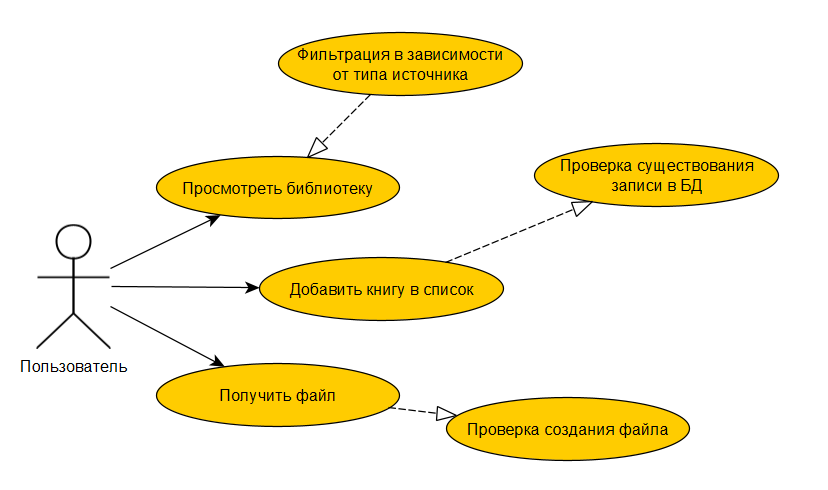
\includegraphics[scale=0.5]{s4Wetlb.png}}
	\caption{Сценарий использования приложения}
	\label{fig:image31}
\end{figure}

\subsection*{Проектирование таблиц базы данных}%
\addcontentsline{toc}{subsection}{\tocsecindent{Проектирование таблиц базы данных}}

База данных приложения состоит из следующих таблиц:
\begin{enumerate}
	\item таблица издателей {\bf publisher};
	\item таблица авторов {\bf author};
	\item таблица книг {\bf book};
	\item таблица нормативно-правовых документов {\bf regulatory\_doc};
	\item таблица нормативно-технических документов {\bf regulatory\_tech\_doc};
		\item таблица авторских свидетельств, патентов {\bf patent};
			\item таблица информационных листков {\bf info\_sheet};
				\item таблица многотомных изданий {\bf multi\_volume};
					\item таблица диссертаций {\bf not\_published\_yet};
						\item таблица электронных ресурсов локального доступа (CD) {\bf elec\_local};
							\item таблица электронный ресурсов удаленного доступа (Internet) {\bf elec\_internet};
								\item таблица статей из книг {\bf book\_article};
										\item таблица статей из газет {\bf newspaper\_article};
											\item таблица рецензий {\bf review};
							
\end{enumerate}

\hfill \break

{\bf Таблица publisher}

Таблица, содержащая информацию об издателях. С помощью связи <<один-к-одному>> связана почти со всеми остальными таблицами БД.

Таблица содержит следующие поля:
\begin{enumerate}
	\item id - целочисленное поле, идентификационный номер издателя;
	\item name - символьное поле, название издателя;
	\item place\_of\_ed – город издательства;
	\item extra\_ed\_info  – дополнительная информация об издательстве.
\end{enumerate}

\hfill \break

{\bf Таблица author}

Таблица, содержащая информацию об авторах. С помощью связи <<один-к-одному>> связана почти со всеми остальными таблицами БД.

Таблица содержит следующие поля:
\begin{enumerate}
	\item id - целочисленное поле, идентификационный номер автора;
	\item name - символьное поле, имя автора;
	\item extra\_info – символьное поле, дополнительная информация об авторе.
\end{enumerate}

\hfill \break

{\bf Таблица book}

Позволяет однозначно описать источник информации, являющийся книгой. Имеет связь <<один-ко-многим>> с таблицами author и publisher. 


Таблица содержит следующие поля:
\begin{enumerate}
	\item id - целочисленное поле, идентификационный номер источника;
	\item name - символьное поле, название источника;
	\item author\_amount - целочисленное поле, обозначающее количество авторов у источника;
	\item first\_author - целочисленное поле, идентификационный номер первого автора;
	\item second\_author - целочисленное поле, идентификационный номер второго автора;
	\item third\_author - целочисленное поле, идентификационный номер третьего автора;
	\item fourth\_author - целочисленное поле, идентификационный номер четвертого автора;
	\item extra\_info - символьное поле, содержащее дополнительную информацию о источнике;
	\item publisher\_id - целочисленное поле, идентификационный номер издателя;
	\item year - целочисленное поле, обозначающее год издания источника;
	\item pages - целочисленное поле, обозначающее количество страниц источника.
\end{enumerate}

\hfill \break

{\bf Таблица regulatory\_doc}

Позволяет однозначно описать источник информации, являющийся нормативно-правовым документом. Имеет связь <<один-ко-многим>> с таблицей publisher. 


Таблица содержит следующие поля:
\begin{enumerate}
	\item id - целочисленное поле, идентификационный номер источника;
	\item name - символьное поле, название источника;
	\item extra\_info - символьное поле, содержащее дополнительную информацию о источнике;
	\item publisher\_id - целочисленное поле, идентификационный номер издателя;
	\item year - целочисленное поле, обозначающее год издания источника;
	\item journal\_id - целочисленное поле, обозначающее номер журнала, в котором был опубликован документ;
	\item first\_page - целочисленное поле, обозначающее первую страницу документа;
	\item last\_page - целочисленное поле, обозначающее последнюю страницу документа.
\end{enumerate}

\hfill \break

{\bf Таблица regulatory\_tech\_doc}

Позволяет однозначно описать источник информации, являющийся нормативно-техническим документом. Имеет связь <<один-ко-многим>> с таблицей publisher. 


Таблица содержит следующие поля:
\begin{enumerate}
	\item id - целочисленное поле, идентификационный номер источника;
	\item name - символьное поле, название источника;
	\item extra\_info - символьное поле, содержащее дополнительную информацию о источнике;
	\item date - поле даты, указывающее дату принятия документа;
	\item publisher\_id - целочисленное поле, идентификационный номер издателя;
	\item year - целочисленное поле, обозначающее год издания источника;
	\item pages - целочисленное поле, обозначающее количество страниц документа.
\end{enumerate}

\hfill \break

{\bf Таблица patent}

Позволяет однозначно описать источник информации, являющийся патентом. Имеет связь <<один-ко-многим>> с таблицами author и publisher. 


Таблица содержит следующие поля:
\begin{enumerate}
	\item id - целочисленное поле, идентификационный номер источника;
	\item name - символьное поле, название источника;
	\item author\_amount - целочисленное поле, обозначающее количество авторов у источника;
	\item first\_author - целочисленное поле, идентификационный номер первого автора;
	\item second\_author - целочисленное поле, идентификационный номер второго автора;
	\item third\_author - целочисленное поле, идентификационный номер третьего автора;
	\item fourth\_author - целочисленное поле, идентификационный номер четвертого автора;
	\item publisher\_id - целочисленное поле, идентификационный номер издателя;
	\item journal\_id - целочисленное поле, обозначающее номер журнала, в котором был опубликован документ;
	\item year - целочисленное поле, обозначающее год издания источника;
	\item pages - целочисленное поле, обозначающее количество страниц источника.
\end{enumerate}
\hfill \break

{\bf Таблица info\_sheet}

Позволяет однозначно описать источник информации, являющийся информационным листком. Имеет связь <<один-ко-многим>> с таблицами author и publisher. 


Таблица содержит следующие поля:
\begin{enumerate}
	\item id - целочисленное поле, идентификационный номер источника;
	\item name - символьное поле, название источника;
	\item author\_amount - целочисленное поле, обозначающее количество авторов у источника;
	\item first\_author - целочисленное поле, идентификационный номер первого автора;
	\item second\_author - целочисленное поле, идентификационный номер второго автора;
	\item third\_author - целочисленное поле, идентификационный номер третьего автора;
	\item fourth\_author - целочисленное поле, идентификационный номер четвертого автора;
	\item publisher\_id - целочисленное поле, идентификационный номер издателя;
	\item year - целочисленное поле, обозначающее год издания источника;
	\item pages - целочисленное поле, обозначающее количество страниц источника.
\end{enumerate}
\hfill \break

{\bf Таблица multi\_volume}

Позволяет однозначно описать источник информации, являющийся многотомным изданием. Имеет связь <<один-ко-многим>> с таблицами author и publisher. 


Таблица содержит следующие поля:
\begin{enumerate}
	\item id - целочисленное поле, идентификационный номер источника;
	\item name - символьное поле, название источника;
	\item author\_amount - целочисленное поле, обозначающее количество авторов у источника;
	\item first\_author - целочисленное поле, идентификационный номер первого автора;
	\item second\_author - целочисленное поле, идентификационный номер второго автора;
	\item third\_author - целочисленное поле, идентификационный номер третьего автора;
	\item fourth\_author - целочисленное поле, идентификационный номер четвертого автора;
	\item extra\_info - символьное поле, содержащее дополнительную информацию о источнике;
	\item publisher\_id - целочисленное поле, идентификационный номер издателя;
	\item year - целочисленное поле, обозначающее год издания источника;
	\item amount\_of\_vols - целочисленное поле, обозначающее количество томов источника.
\end{enumerate}

\hfill \break

{\bf Таблица not\_published\_yet}

Позволяет однозначно описать источник информации, являющийся диссертацией. Имеет связь <<один-ко-многим>> с таблицами author и publisher. 


Таблица содержит следующие поля:
\begin{enumerate}
	\item id - целочисленное поле, идентификационный номер источника;
	\item name - символьное поле, название источника;
	\item author - целочисленное поле, идентификационный номер автора;
	\item date - поле даты, указывающее дату защиты документа;
	\item date - поле даты, указывающее дату утверждения документа;
	\item extra\_info - символьное поле, содержащее дополнительную информацию о источнике;
	\item publisher\_id - целочисленное поле, идентификационный номер издателя;
	\item year - целочисленное поле, обозначающее год издания источника.
\end{enumerate}

\hfill \break

{\bf Таблица elec\_local}

Позволяет однозначно описать источник информации, являющийся электронным ресурсом локального доступа (CD). Имеет связь <<один-ко-многим>> с таблицами author и publisher. 


Таблица содержит следующие поля:
\begin{enumerate}
	\item id - целочисленное поле, идентификационный номер источника;
	\item name - символьное поле, название источника;
	\item author\_amount - целочисленное поле, обозначающее количество авторов у источника;
	\item first\_author - целочисленное поле, идентификационный номер первого автора;
	\item second\_author - целочисленное поле, идентификационный номер второго автора;
	\item third\_author - целочисленное поле, идентификационный номер третьего автора;
	\item fourth\_author - целочисленное поле, идентификационный номер четвертого автора;
	\item extra\_info - символьное поле, содержащее дополнительную информацию о источнике;
	\item type - символьное поле, обозначающее тип ресурса;
	\item publisher\_id - целочисленное поле, идентификационный номер издателя;
	\item year - целочисленное поле, обозначающее год издания источника;
	\item material\_desc - символьное поле, обозначающее информацию о материале источника.
\end{enumerate}

\hfill \break

{\bf Таблица elec\_internet}

Позволяет однозначно описать источник информации, являющийся электронным ресурсом удаленного доступа (Internet). Имеет связь <<один-ко-многим>> с таблицами author и publisher. 


Таблица содержит следующие поля:
\begin{enumerate}
	\item id - целочисленное поле, идентификационный номер источника;
	\item name - символьное поле, название источника;
	\item author\_amount - целочисленное поле, обозначающее количество авторов у источника;
	\item first\_author - целочисленное поле, идентификационный номер первого автора;
	\item second\_author - целочисленное поле, идентификационный номер второго автора;
	\item third\_author - целочисленное поле, идентификационный номер третьего автора;
	\item fourth\_author - целочисленное поле, идентификационный номер четвертого автора;
	\item extra\_info - символьное поле, содержащее дополнительную информацию о источнике;
	\item publisher\_id - целочисленное поле, идентификационный номер издателя;
	\item year - целочисленное поле, обозначающее год издания источника;
	\item url - символьное поле, содержащее ссылку на ресурс.
\end{enumerate}

\hfill \break

{\bf Таблица book\_article}

Позволяет однозначно описать источник информации, статьей из книги. Имеет связь <<один-ко-многим>> с таблицами author, book и publisher. 


Таблица содержит следующие поля:
\begin{enumerate}
	\item id - целочисленное поле, идентификационный номер источника;
	\item name - символьное поле, название источника;
	\item author\_amount - целочисленное поле, обозначающее количество авторов у источника;
	\item first\_author - целочисленное поле, идентификационный номер первого автора;
	\item second\_author - целочисленное поле, идентификационный номер второго автора;
	\item third\_author - целочисленное поле, идентификационный номер третьего автора;
	\item fourth\_author - целочисленное поле, идентификационный номер четвертого автора;
	\item extra\_info - символьное поле, содержащее дополнительную информацию о источнике;
	\item book\_id - целочисленное поле, идентификационный номер книги;
	\item year - целочисленное поле, обозначающее год издания источника;
	\item page - целочисленное поле, обозначающее номер страницы статьи.
\end{enumerate}

\hfill \break

{\bf Таблица newspaper\_article}

Позволяет однозначно описать источник информации, являющийся  статьей из газеты. Имеет связь <<один-ко-многим>> с таблицами author, book и publisher. 


Таблица содержит следующие поля:
\begin{enumerate}
	\item id - целочисленное поле, идентификационный номер источника;
	\item name - символьное поле, название источника;
	\item author\_amount - целочисленное поле, обозначающее количество авторов у источника;
	\item first\_author - целочисленное поле, идентификационный номер первого автора;
	\item second\_author - целочисленное поле, идентификационный номер второго автора;
	\item third\_author - целочисленное поле, идентификационный номер третьего автора;
	\item fourth\_author - целочисленное поле, идентификационный номер четвертого автора;
	\item extra\_info - символьное поле, содержащее дополнительную информацию о источнике;
	\item newspaper\_name - символьное поле, содержащее название газеты;
	\item newspaper\_year - целочисленное поле, обозначающее год издания газеты;
	\item newspaper\_number - целочисленное поле, обозначающее номер газеты;
	\item year - целочисленное поле, обозначающее год издания источника;
	\item page - целочисленное поле, обозначающее номер страницы статьи.
\end{enumerate}

\hfill \break

{\bf Таблица review}

Позволяет однозначно описать источник информации, являющийся  реценщией. Имеет связь <<один-ко-многим>> с таблицами author, book и publisher. 


Таблица содержит следующие поля:
\begin{enumerate}
	\item id - целочисленное поле, идентификационный номер источника;
	\item name - символьное поле, название источника;
	\item author\_amount - целочисленное поле, обозначающее количество авторов у источника;
	\item first\_author - целочисленное поле, идентификационный номер первого автора;
	\item second\_author - целочисленное поле, идентификационный номер второго автора;
	\item third\_author - целочисленное поле, идентификационный номер третьего автора;
	\item fourth\_author - целочисленное поле, идентификационный номер четвертого автора;
	\item extra\_info - символьное поле, содержащее дополнительную информацию о источнике;
	\item journal\_name - символьное поле, содержащее название журнала;
	\item journal\_year - целочисленное поле, обозначающее год издания журнала;
	\item journal\_number - целочисленное поле, обозначающее номер журнала;
	\item year - целочисленное поле, обозначающее год издания источника;
	\item page - целочисленное поле, обозначающее номер страницы статьи.
\end{enumerate}


\newpage
\begin{figure}[h!]
	\center{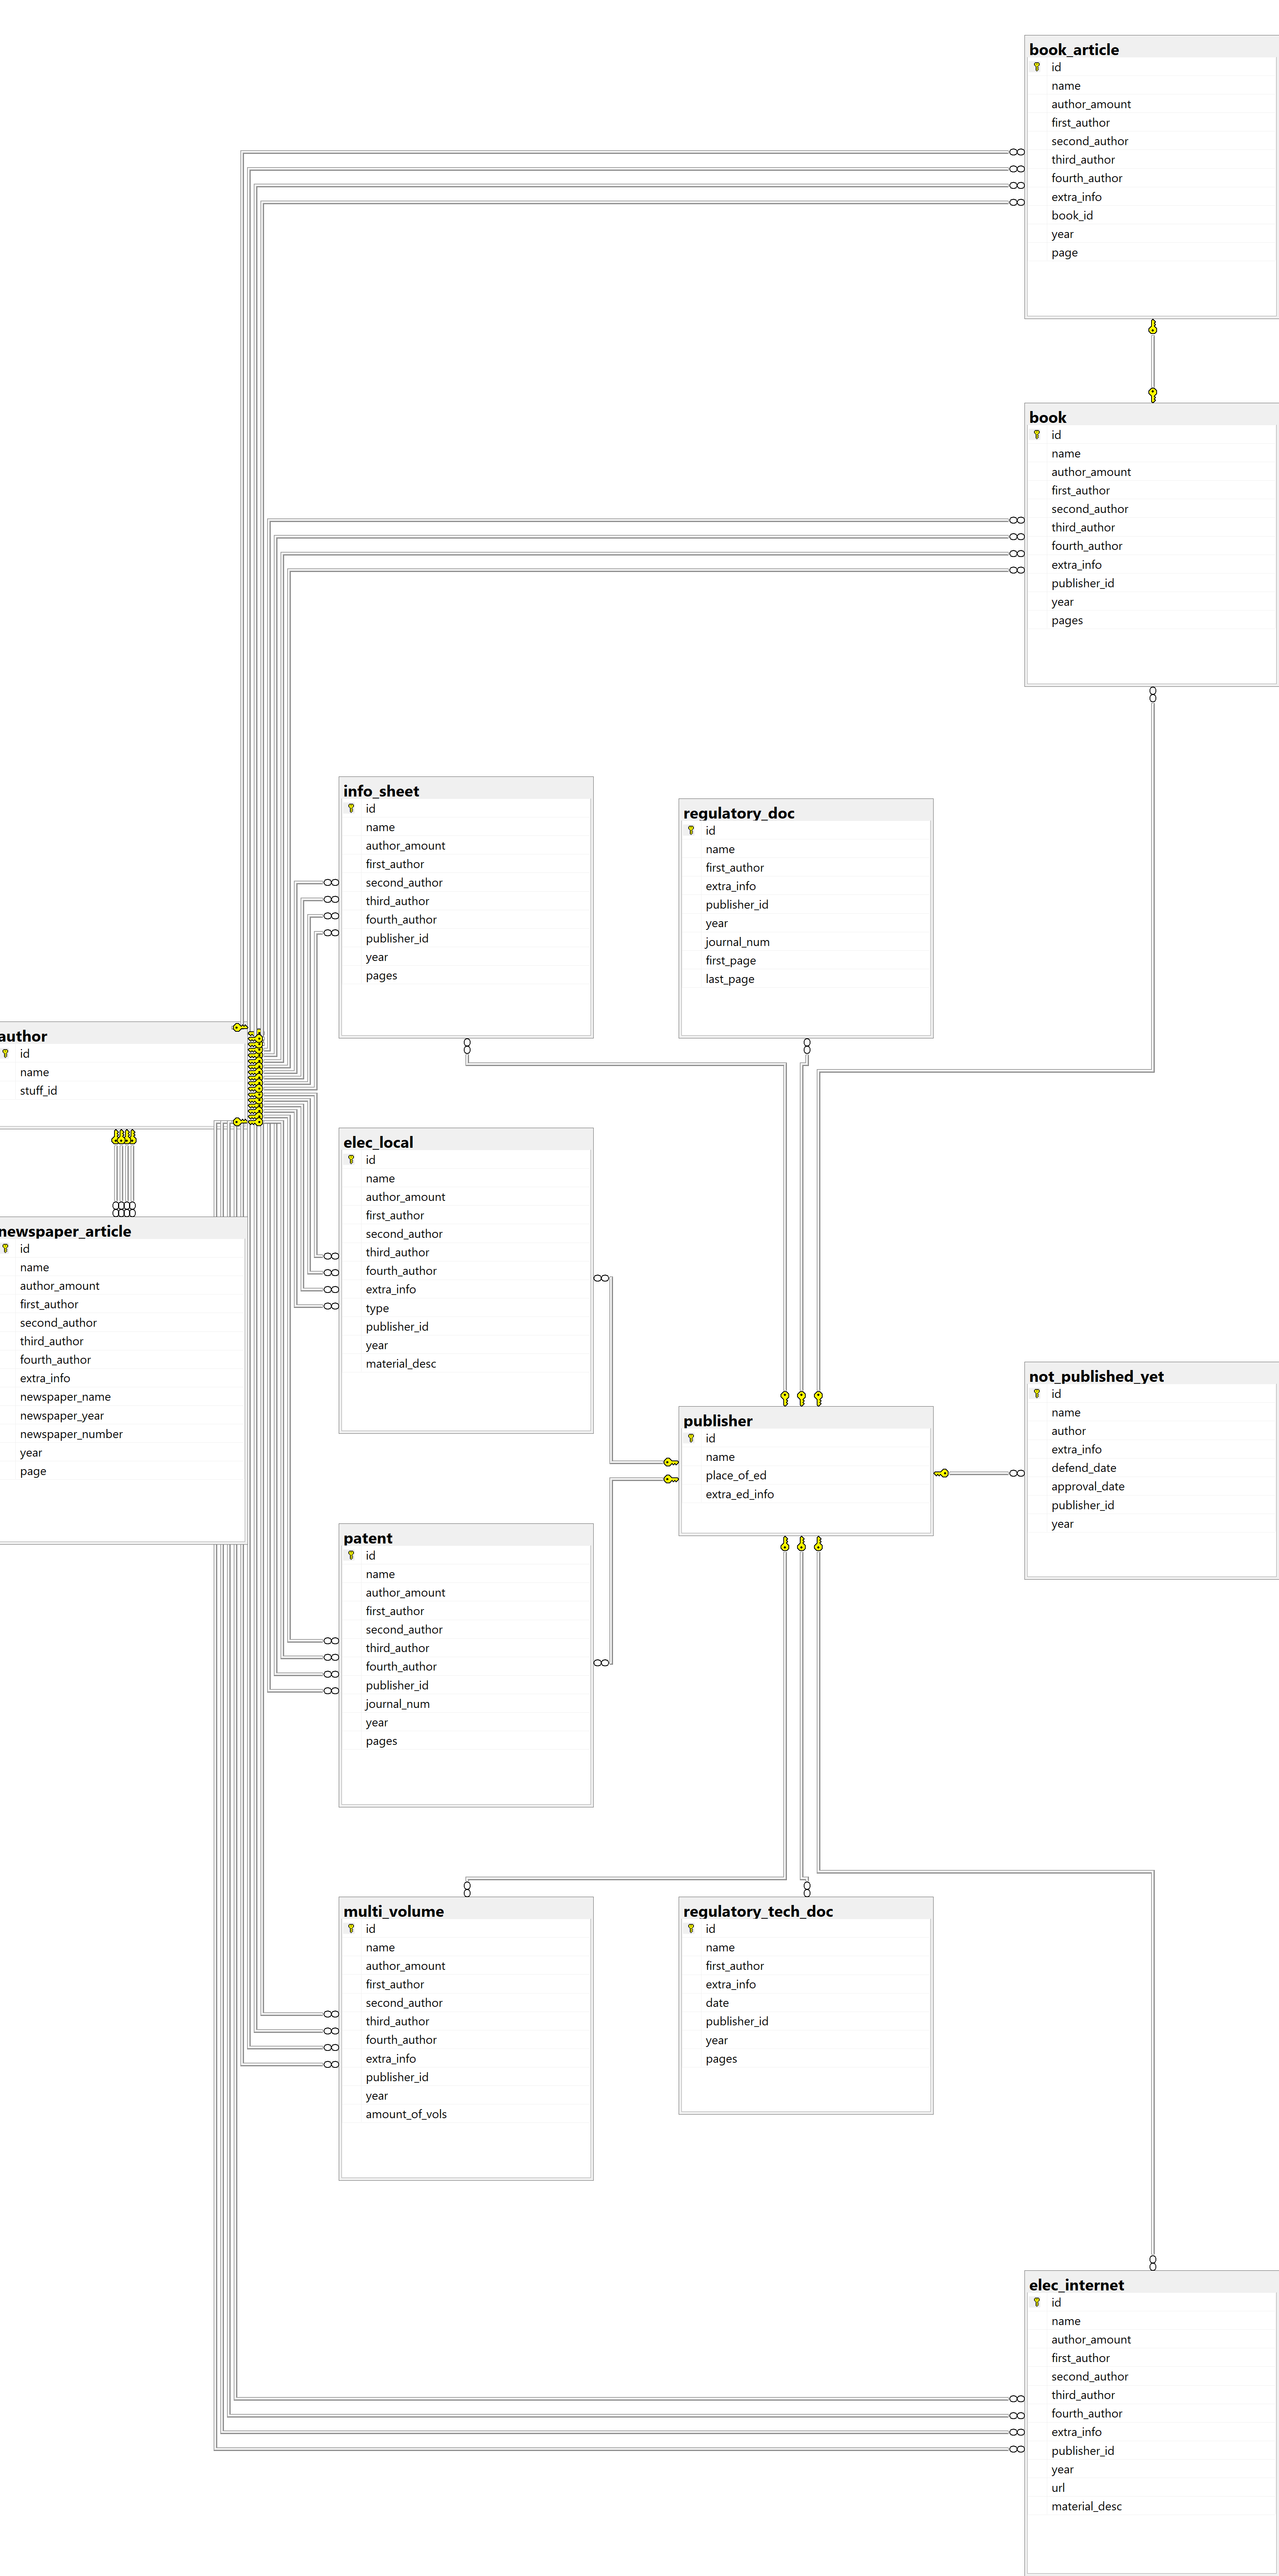
\includegraphics[scale=0.17]{bd.png}}
	\caption{Диаграмма БД}
	\label{fig:image1}
\end{figure}


\subsection*{Проектирование системы доступа к данных}%
\addcontentsline{toc}{subsection}{\tocsecindent{Проектирование системы получения данных}}
Для обеспечения доступа к данных будем использовать библиотеку pyodbc для Python, отправляя SQL запросы в нашу БД. 

Создание web-интерфейса будет реализовано с помощью фреймворка Dash. Приложения Dash должны состоять из двух частей: layout (то, что будет выведено на экран) и самого кода программы.

Фреймворк Dash предоставляет собой набор данных базовых инструментов для реализации web-приложения, поэтому интерфейс будет создан с помощью уже готовых средств.

\subsection*{Вывод}%
\addcontentsline{toc}{subsection}{\tocsecindent{Вывод}}
Была разработана модель приложения, дающего возможность генерировать список литературы для среды LaTeX.

%%%%%%%%%%%%%%%%%%%%%%%%%%%%%%%%%%%%%%%%%%%%%%%%%%%%%%%%%%%%%%%%%%%%%

\newpage
\section*{Технологическая часть}%
\addcontentsline{toc}{section}{\tocsecindent{Технологическая часть}}

После проектирования структуры поставленной задачи, требуется реализовать набор функций, необходимый для создания web-приложения, а также конкретизировать полный список инструментов, используемых для запуска приложения.

\subsection*{Выбор инструментов разработки}%
\addcontentsline{toc}{subsection}{\tocsecindent{Выбор инструментов разработки}}

В ходе реализации были использованы следующие технологии и средства:

\begin{itemize}
	\item язык программирования Python;
	\item СУБД MS-SQL;
	\item библиотека pyodbc;
	\item фреймворк Dash.
\end{itemize}

Такой набор инструментов был выбран в связи с тем, что для каждого из элементов предусмотрено взаимодействие с другими. Помимо этого, данные инструменты полностью выполняют задачи, необходимые для реализации проекта.

Для разработки и тестирования приложения был использован компьютер с операционной системой Windows 10.

\subsection*{Реализация доступа к данным}%
\addcontentsline{toc}{subsection}{\tocsecindent{Реализация доступа к данным}}

Для работы с базой данных для начала требуется установить соединение.

\begin{lstlisting}[label=some-code1, caption=Подключение к БД]
print("Идет загрузка БД, пожалуйста, подождите...")

cnxn = pyodbc.connect(driver='{SQL Server}', Server='DESKTOP-IEVL6PF', database='course_project',
trusted_connection='yes')
cursor = cnxn.cursor()

print("БД была успешно загружена")

cursor.execute("select * from book")
books = cursor.fetchall()
\end{lstlisting}

Ниже представлено получение данных для просмотра в web-приложении в зависимости от выбранной категории.
\begin{lstlisting}[label=some-code2, caption=Получение данных из таблиц]
@app.callback(Output('table', 'data'),
[Input('input3', 'value')]
)
def load_table(value):
	global cursor, columns_of_books

	if value == '1':

		cursor.execute("select id, name, first_author, year, extra_info from book")
		books = cursor.fetchall()
		
		return [dict(zip(columns_of_books, d)) for d in books]

	if value == '2':

		cursor.execute("select id, name, first_author, year, extra_info from regulatory_doc")
		books = cursor.fetchall()

		return [dict(zip(columns_of_books, d)) for d in books]
...
\end{lstlisting}

\subsection*{Реализация обработки данных}%
\addcontentsline{toc}{subsection}{\tocsecindent{Реализация обработки данных}}

Для работы с данными потребовалось реализовать несколько различных функций из-за отличий в правилах оформления для каждого источника.

Ниже представлена функция обработки книг в правильный формат.

\begin{lstlisting}[label=some-code2, caption=Обработка данных]
def print_books(input_str):
	global cursor, str_to_write, counter

	cursor.execute("select * from book where name = 	'{}'".format(input_str))
	book = cursor.fetchall()
	str_to_write += "\n\\bibitem{{litlink{}}} ".format(counter)

	counter += 1
	amount_of_authors = book[0][2]

	if amount_of_authors == 1:
	str_to_write += u"{}. {} [Текст]".format(book[0][3], book[0][1])
	if book[0][7] != None:
		str_to_write += u": {} / {} - {}: {}, {}. - {} с.".format(book[0][7], book[0][3], book[0][8], book[0][10],
				book[0][11], book[0][12])
	else:
		str_to_write += u" / {} - {}: {}, {}. - {} с.".format(book[0][3], book[0][8], book[0][10],
	book[0][11], book[0][12])

	elif amount_of_authors == 2:
		str_to_write += u"{}. {} [Текст]".format(book[0][3], book[0][1])
		if book[0][7] != None:
			str_to_write += u": {} / {}, {} - {}: {}, {}. - {} с.".format(book[0][7], book[0][3], book[0][4], book[0][8], book[0][10],
				book[0][11], book[0][12])
		else:
			str_to_write += u" / {}, {} - {}: {}, {}. - {} с.".format(book[0][3], book[0][4], book[0][8], book[0][10],
			book[0][11], book[0][12])

	elif amount_of_authors == 3:
		str_to_write += u"{}. {} [Текст]".format(book[0][3], book[0][1])
		if book[0][7] != None:
			str_to_write += u": {} / {}, {}, {} - {}: {}, {}. - {} 		с.".format(book[0][7], book[0][3], book[0][4],
			book[0][5], book[0][8], book[0][10],
			book[0][11], book[0][12])
		else:
			str_to_write += u" / {}, {}, {} - {}: {}, {}. - {} с.".format(book[0][3], book[0][4], book[0][5],
			book[0][8], book[0][10],
			book[0][11], book[0][12])
	elif amount_of_authors == 4:
		str_to_write += u"{}. {} [Текст]".format(book[0][3], book[0][1])
		if book[0][7] != None:
			str_to_write += u": {} / {}, {}, {}, {} - {}: {}, {}. - {} с.".format(book[0][7], book[0][3], book[0][4],
			book[0][5], book[0][6],book[0][8], book[0][10],
			book[0][11], book[0][12])
		else:
			str_to_write += u" / {}, {}, {}, {}  - {}: {}, {}. - {} с.".format(book[0][3], book[0][4], book[0][5],
			book[0][6],book[0][8], book[0][10],
			book[0][11], book[0][12])

\end{lstlisting}
\subsection*{Frontend-разработка}%
\addcontentsline{toc}{subsection}{\tocsecindent{Реализация доступа к данным}}
Чтобы обеспечить доступ к данным нужно создать форму, позволяющую отображать записи в таблицах. В Dash для этого используется класс dash\_table.DataTable. Поскольку таблица может меняться в зависимости от ресурса, потребовалось использовать параметр editable=True.

Для выбора типа источника данных использовался класс dcc.Dropdown, для ввода - dcc.Input. \cite{4}

\begin{lstlisting}[label=some-code, caption=Форма добавления книги]
app = dash.Dash(__name__, external_stylesheets=external_stylesheets)

	app.layout = html.Div([
	html.H1(
			children='Курсовой проект,',
			style={
			'textAlign': 'center',
			'color': '#7FDBFF'}
	),

	html.Div(
			children='позволяющий сформировать список литературы для TeX', 
			style={
			'textAlign': 'center',
			'color': '#7FDBFF'}
		),

	html.Label('Для начала следует создать файл:'),
	html.Button(children = 'Создать файл', id='first_button', n_clicks = 0),
	html.Div(id="output0", children=' '),

	html.Label('Введите название желаемой книги/документа/статьи etc.:'),
	dcc.Input(id = 'input1', type='text'),

	html.Label('Выберите тип источника:'),
	dcc.Dropdown(id = 'input2',
	options=[
	{'label': u'Книга', 'value': '1'},
	{'label': u'Нормативно-правовой документ', 'value': '2'},
	{'label': u'Нормативно-технический документ', 'value': '3'},
	{'label': u'Авторское свидетельство, патент', 'value': '4'},
	{'label': u'Информационные листки', 'value': '5'},
	{'label': u'Многотомные издания', 'value': '6'},
	{'label': u'Диссертации', 'value': '7'},
	{'label': u'Электронный ресурс локального доступа (CD)', 'value': '8'},
	{'label': u'Электронный ресурс удаленного доступа (Internet)', 	'value': '9'},
	{'label': u'Статья из книги', 'value': '10'},
	{'label': u'Статья  из журнала', 'value': '11'},
	{'label': u'Рецензия', 'value': '12'}
	]
	),
	
	html.Br(),
	html.Button(children = 'Добавить книгу', id='button', n_clicks 	= 0),
	html.Div(id="output", children=' '),

	html.Label('После того, как все книги добавлены:'),
	html.Button(children = 'Получить файл', id='last_button', 	n_clicks = 0),
	html.Div(id="output2", children=' '),
	html.Br(),
	html.Label('Тут можно посмотреть, что есть в БД:'),
	dcc.Dropdown(id = 'input3',
	options=[
	{'label': u'Книга', 'value': '1'},
	{'label': u'Нормативно-правовой документ', 'value': '2'},
	{'label': u'Нормативно-технический документ', 'value': '3'},
	{'label': u'Авторское свидетельство, патент', 'value': '4'},
	{'label': u'Информационные листки', 'value': '5'},
	{'label': u'Многотомные издания', 'value': '6'},
	{'label': u'Диссертации', 'value': '7'},
	{'label': u'Электронный ресурс локального доступа (CD)', 'value': '8'},
	{'label': u'Электронный ресурс удаленного доступа (Internet)', 'value': '9'},
	{'label': u'Статья из книги', 'value': '10'},
	{'label': u'Статья  из журнала', 'value': '11'},
	{'label': u'Рецензия', 'value': '12'}
	], value = '1'
	),

	dash_table.DataTable(
	id='table',
	columns=[{"name": i, "id": i} for i in columns_of_books],
	data=[dict(zip(columns_of_books, d)) for d in books],
	editable=True
	)
])

\end{lstlisting}

\subsection*{Интерфейс приложения}%
\addcontentsline{toc}{subsection}{\tocsecindent{Интерфейс приложения}}

На рис. \ref{fig:image3} показан основной интерфейс приложения.

\begin{figure}[h!]
	\center{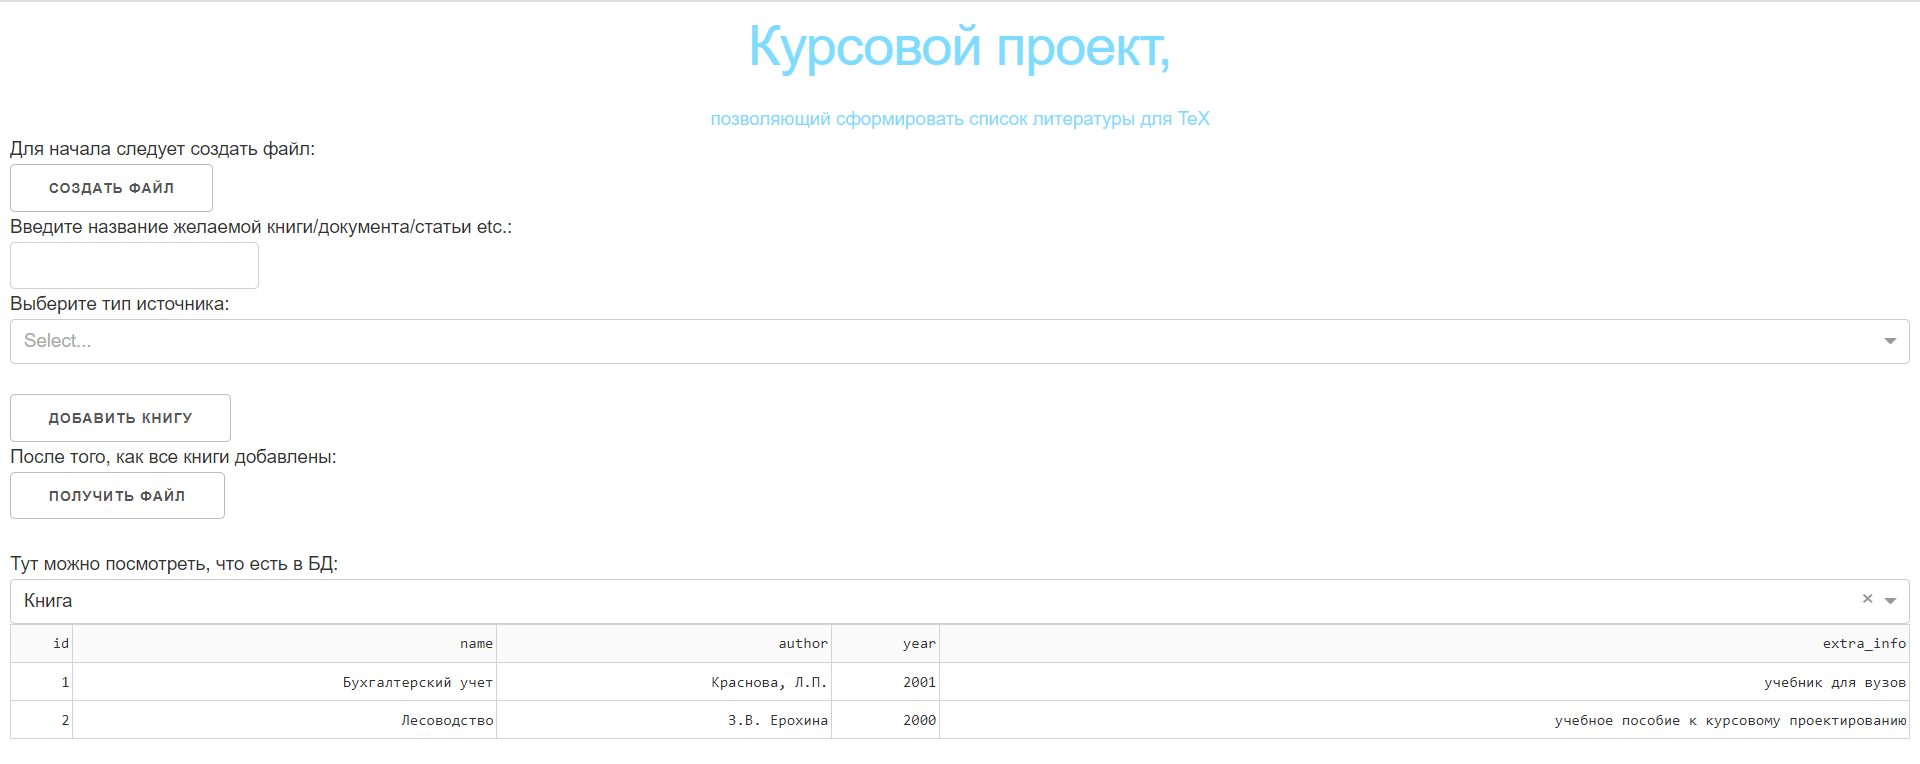
\includegraphics[scale=0.24]{fL43VnK.png}}
	\caption{Интерфейс приложения}
	\label{fig:image3}
\end{figure}

\subsection*{Требования к аппаратуре}%
\addcontentsline{toc}{subsection}{\tocsecindent{Требования к аппаратуре}}

Пользовательский интерфейс представляет из себя одно страничное
приложение для браузера, поэтому взаимодействие с сервисом может осуществляться только через браузер.

\subsection*{Тестирование}%
\addcontentsline{toc}{subsection}{\tocsecindent{Тестирование
}}

Протестируем программу, создав файл в web-приложении:
\begin{figure}[h!]
	\center{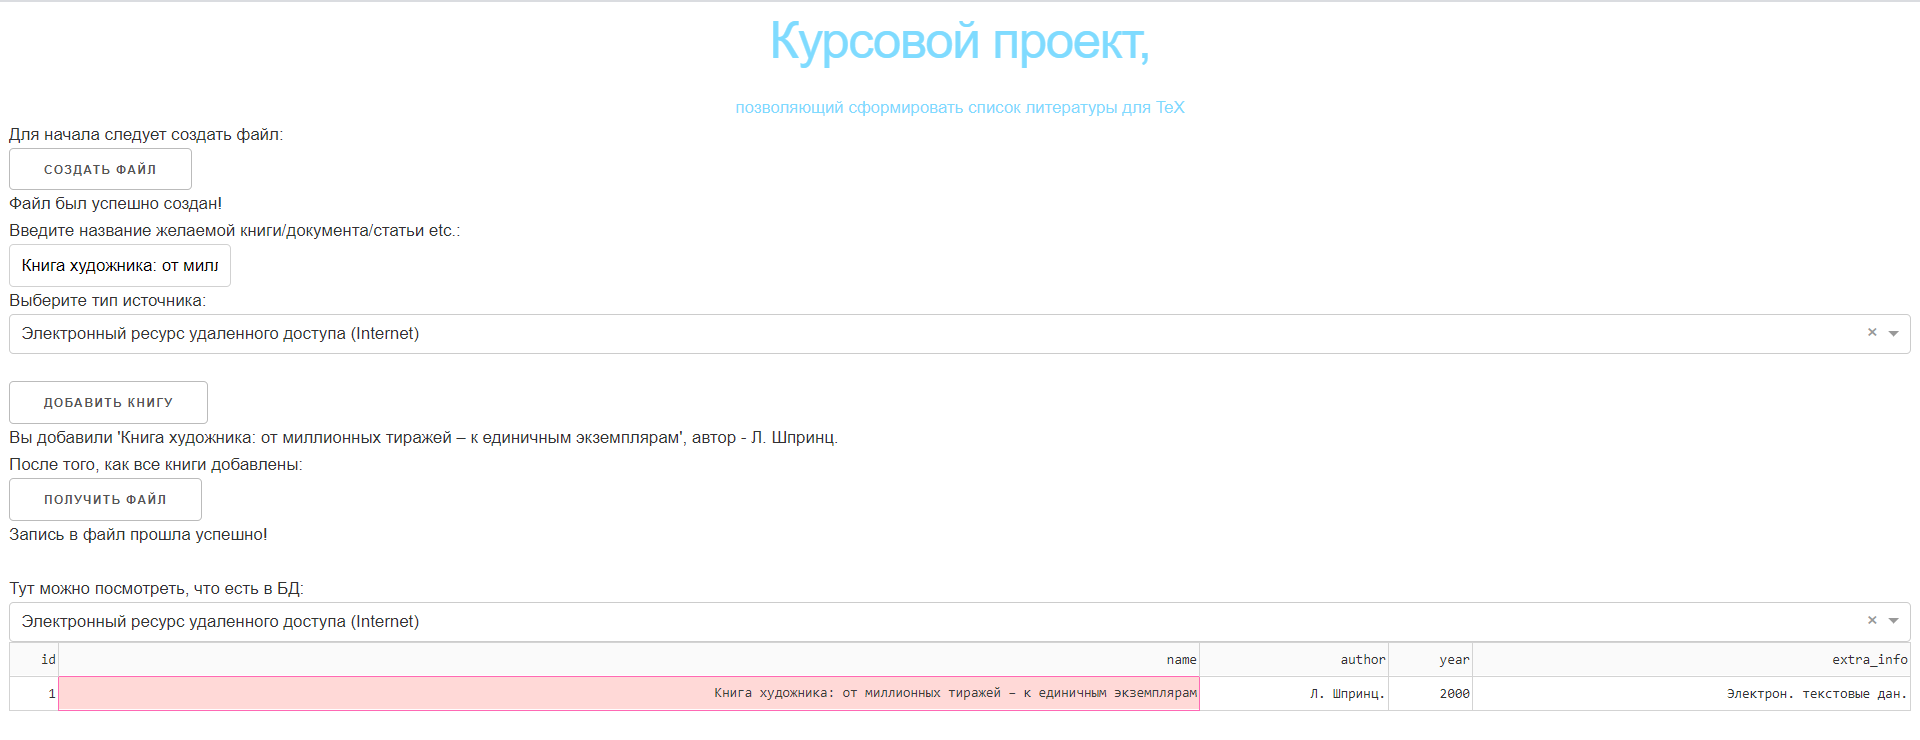
\includegraphics[scale=0.24]{Ty6ZhV2.png}}
	\caption{Демонстрация успешного создания файла}
	\label{fig:image5}
\end{figure}
\newline Тем временем, в папке с программой был действительно появился файл:
\begin{figure}[h!]
	\center{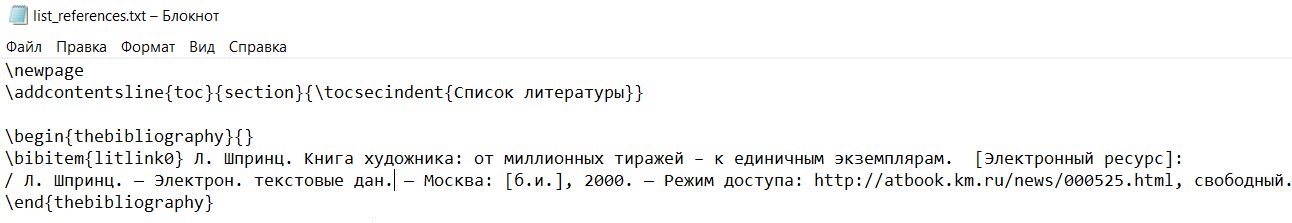
\includegraphics[scale=0.3]{REMefjo.png}}
	\caption{Созданный файл}
	\label{fig:image4}
\end{figure}

Было проведено функциональное тестирование белого ящика, в ходе
которого программа отработала правильно. Помимо этого, было проведено тестирование пользовательского интерфейса, все элементы интерфейса реагируют корректно.
\subsection*{Вывод}%
\addcontentsline{toc}{subsection}{\tocsecindent{Вывод}}
Был реализовано веб-приложение на языке Python. Программа полностью
прошла функциональное тестирование и тестирование интерфейса.
\newpage
\section*{Заключение}%
\addcontentsline{toc}{subsection}{\tocsecindent{Заключение}}
В результате проделанной работы:
\begin{enumerate}
	\item были продуманы функции, которые должно было решать приложение;
	\item проведен анализ инструментов, необходимых для проектирования и реализации задачи, в результате которого были выбраны такие инструменты, как MS-SQL, pyodbc, Dash;
	\item разработана структура базы данных, состоящая из нескольких сущностей;
	\item с помощью выбранных инструментов был реализован и протестирован web-интерфейс, позволяющий создавать файл литературы, а также просматривать содержимое библиотеки.
\end{enumerate}



















